% --------------------------------------------------------------
% This is all preamble stuff that you don't have to worry about.
% Head down to where it says "Start here"
% --------------------------------------------------------------

\documentclass[12pt]{article}

\usepackage[margin=1in]{geometry}
\usepackage{amsmath,amsthm,amssymb}
\usepackage{graphicx} %This allows to include eps figures

% This is to include code
\usepackage{listings}
\usepackage{xcolor}
\definecolor{dkgreen}{rgb}{0,0.6,0}
\definecolor{gray}{rgb}{0.5,0.5,0.5}
\definecolor{mauve}{rgb}{0.58,0,0.82}
\lstdefinestyle{Python}{
    language        = Python,
    basicstyle      = \ttfamily,
    keywordstyle    = \color{blue},
    keywordstyle    = [2] \color{teal}, % just to check that it works
    stringstyle     = \color{green},
    commentstyle    = \color{red}\ttfamily
}

\newcommand{\N}{\mathbb{N}}
\newcommand{\Z}{\mathbb{Z}}

\newenvironment{theorem}[2][Theorem]{\begin{trivlist}
\item[\hskip \labelsep {\bfseries #1}\hskip \labelsep {\bfseries #2.}]}{\end{trivlist}}
\newenvironment{lemma}[2][Lemma]{\begin{trivlist}
\item[\hskip \labelsep {\bfseries #1}\hskip \labelsep {\bfseries #2.}]}{\end{trivlist}}
\newenvironment{exercise}[2][Exercise]{\begin{trivlist}
\item[\hskip \labelsep {\bfseries #1}\hskip \labelsep {\bfseries #2.}]}{\end{trivlist}}
\newenvironment{reflection}[2][Reflection]{\begin{trivlist}
\item[\hskip \labelsep {\bfseries #1}\hskip \labelsep {\bfseries #2.}]}{\end{trivlist}}
\newenvironment{proposition}[2][Proposition]{\begin{trivlist}
\item[\hskip \labelsep {\bfseries #1}\hskip \labelsep {\bfseries #2.}]}{\end{trivlist}}
\newenvironment{corollary}[2][Corollary]{\begin{trivlist}
\item[\hskip \labelsep {\bfseries #1}\hskip \labelsep {\bfseries #2.}]}{\end{trivlist}}

\begin{document}

% --------------------------------------------------------------
%                         Start here
% --------------------------------------------------------------

%\renewcommand{\qedsymbol}{\filledbox}

\title{Homework 2}%replace X with the appropriate number
\author{Thomas Buchegger\\ %replace with your name
Introduction to Signal and Image Processing}
\maketitle

\section*{Abstract}
This report is based on Homework 2 in the course Introduction to Signal and Image Processing. 

\setcounter{tocdepth}3 % Set the depth of the table of contents to show sections and subsections only
\tableofcontents

\pagebreak
\section{Used Methods}
\subsection{Linear Filtering}
Linear filtering is used to modify a picture. This includes enhancing or removing features. Filtering is a so called neighbourhood operation, which means
that the value of a certain pixel is based on its neighbourhood pixels.
\newline
An example for a linear filter would be a box filter. It calculates the arithmetic means
based on its neighbourhood pixels for the new pixel. This leads to a blurring effect. 

\begin{figure}[!htb]
    \centering
    %omit extension of file. pdflatex will convert to pdf automatically.
    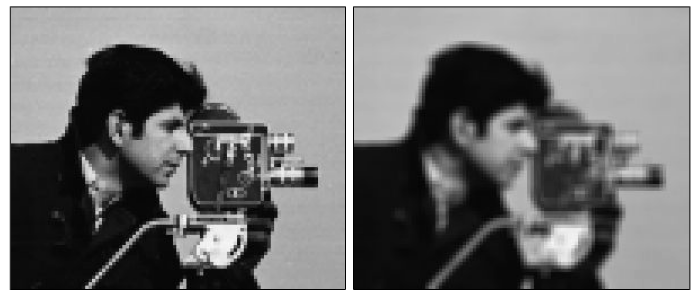
\includegraphics[width=0.8\textwidth]{pics/boxFilterExample}
    \caption{Filtering with a box-filter of size $3 \times 3$.}
    \label{fig:boxfilter}
    \end{figure}

\subsection{Finding edges}
As the name suggests, the goal is to detect edges in images.
One of the most popular edge detection algorithm is canny edge detection.
\newline
It consists of four steps:
\begin{enumerate}  
    \item Preprocessing with gauss for example
    \begin{figure}[!htb]
         \centering
         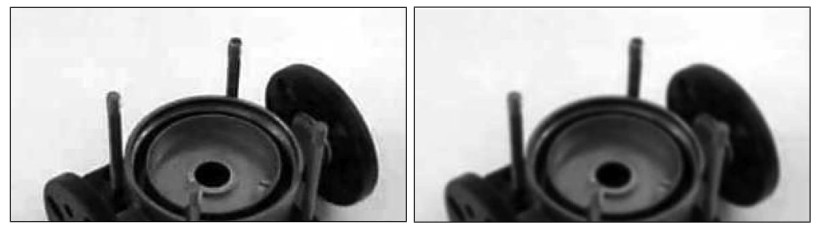
\includegraphics[width=0.8\textwidth]{pics/canny1}
         \caption{Before and after low pass filter}
    \end{figure}

    \item Gradient calculation
    \begin{figure}[!htb]
        \centering
        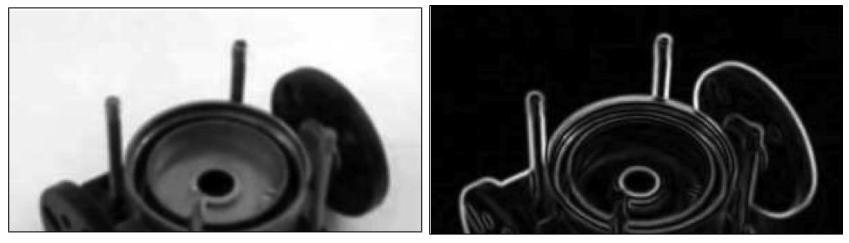
\includegraphics[width=0.8\textwidth]{pics/canny2}
        \caption{Before and after gradient calculation}
    \end{figure}

    \item Nonmax suppression
    \begin{figure}[!htb]
        \centering
        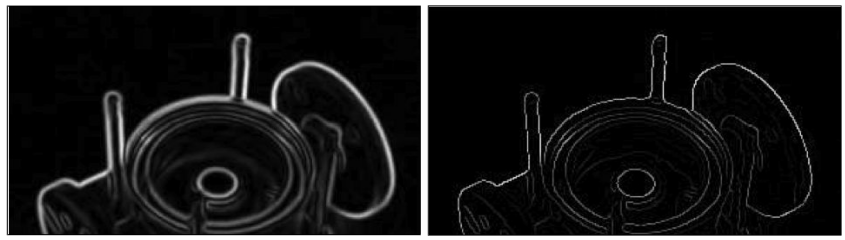
\includegraphics[width=0.8\textwidth]{pics/canny3}
        \caption{Before and after non max suppression}  
    \end{figure}

    \item Hysteresis thresholding
    \begin{figure}[!htb]
        \centering
        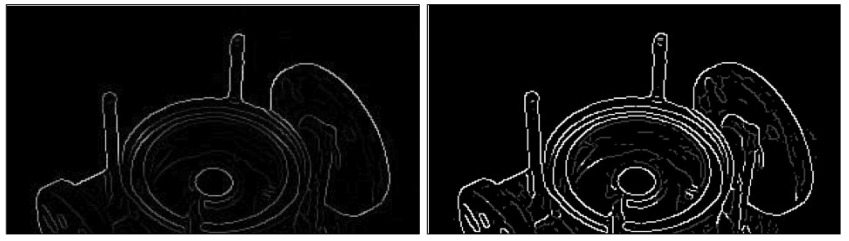
\includegraphics[width=0.8\textwidth]{pics/canny4}
        \caption{Before and after thresholding}
    \end{figure}

    \end{enumerate}

\subsection{Corner detection}
The goal is to detect corners in images. A corner is defined as an intersection
between two edges. 

\section{Exercises}
\subsection{Linear Filtering}
\subsubsection{Boxfilter}
The function boxfilter(n) can be summarized as $np.ones((n, n)) / (n x n)$.


\subsubsection{myconv2}


\subsubsection{boxfilter with myconv2}
\subsubsection{gauss1d}
\subsubsection{gauss2d}
\subsubsection{gconv}
\subsubsection{More efficient convolution}
 

\subsubsection{Computation time vs filter size experiment}

\subsection{Finding edges}
\subsubsection{gradients}
Gradient detection is done with a high pass filter. In our excercise this is done with
once in x and once in y direction with the help of the $myconv2$ and $gauss1d$ functions.
The value for sigma is 1. 

\subsubsection{create edge magn image}

\begin{figure}[!htb]
    \centering
    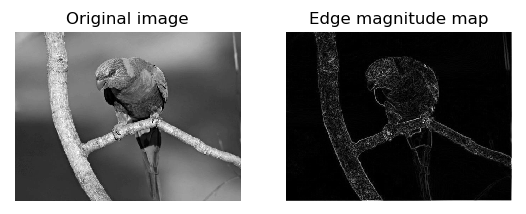
\includegraphics[width=0.8\textwidth]{pics/edgeMagnitudeMap}
    \caption{Original image and its magnitude map}
\end{figure}

\subsubsection{make edge map}


\subsubsection{edge non max suppression}
The non max suppression is the last step of the canny edge detector algorithm.
This step is needed, bceause edges are usually larger than one pixel, so they
get reduced to the pixel with the max. gradient.
\newline
This is done by iterating through the picture four times, once in each direction. 
The currently looked at pixel is then compared to its neighbours. If it has the
strongest gradient in [x,y], then it survives. Else it's set to 0.

\begin{figure}[!htb]
    \centering
    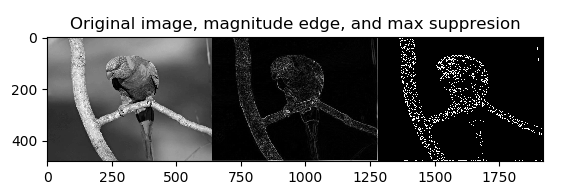
\includegraphics[width=0.8\textwidth]{pics/origMagNonMax}
    \caption{Comparison of original image, image with gradients and image with non max suppression}
\end{figure}


\subsection{Corner detection}
\subsubsection{myharris}
\subsubsection{Evaluate myharris}
\subsubsection{Evaluate myharris rot 45}
\subsubsection{Evaluate myharris downscaled}
\subsubsection{}

\pagebreak


\end{document}